\section{Why the discrete and continuous constants differ}
\label{a:sec:compare}

The two quasi-stationary constants now in hand are
\begin{equation*}
\Ac(p) = \frac{1-2p}{1-p}\quad\text{(continuous time)},
\qquad
A(p) = \lim_{n\to\infty}\frac{S_n}{(2p)^n}\quad\text{(discrete time)},
\end{equation*}
and the observation that organises this section is that the first starts at $1$
where the second starts at $\tfrac12$, yet halving the first does not superpose
the curves (\cref{a:fig:dtct}).

\begin{figure}[ht]
\centering
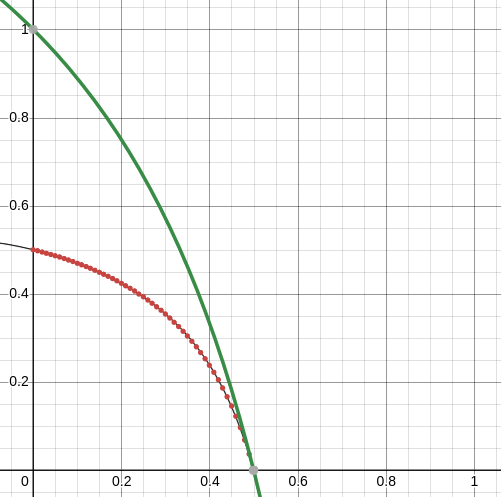
\includegraphics[width=0.5\textwidth]{figures/dtctA.png}
\caption{The elementary continuous-time constant $\Ac(p) = (1-2p)/(1-p)$ (green)
against high-precision numerical values of the discrete-time constant $A(p)$ (red
points). Both vanish at $p=\tfrac12$, but at $p=0$ the continuous curve starts at
$1$ and the discrete one at $\tfrac12$, and the two are not related by a constant
factor in between. The black line is one of the fitted surrogates produced by the
symbolic-regression search of \cref{a:sec:GA}; it tracks the points closely but is
not exact.}
\label{a:fig:dtct}
\end{figure}

\Cref{a:prop:bounds} explains this completely. What holds is not
$A=\tfrac12\Ac$ but the strict inequality $A>\tfrac12\Ac$, and the inequality is
attained only in the limit $p\to0$. Combining \cref{a:eq:Aasym} with the
elementary form of $\Ac$, the ratio runs across the interval with the endpoint
limits
\begin{equation}
\label{a:eq:ratiolimits}
\frac{A(p)}{\Ac(p)} \;\longrightarrow\; \tfrac12 \quad(p\to0),
\qquad
\frac{A(p)}{\Ac(p)} \;\longrightarrow\; 1 \quad(p\to\tfrac12^-),
\end{equation}
taking the values $0.503$, $0.528$, $0.619$, $0.798$, $0.928$ and $0.988$ at
$p=0.01,\,0.1,\,0.3,\,0.45,\,0.49,\,0.499$. The computed ratios increase
monotonically through this list; that monotonicity is descriptive, and no
monotonicity theorem is needed for \cref{a:eq:ratiolimits}. No constant factor
will do, because the ratio is not constant.

The two endpoints have clean interpretations, and they are different in kind.

At $p\to0$ the factor of two is a counting effect. In the binary discrete model an
individual leaves either nothing or two offspring, so a surviving population is
always even (\cref{a:prop:parity}); deep in the subcritical regime, conditioning on
survival means conditioning on a population of exactly two, and the
quasi-stationary mean is $2$. In the continuous-time model a survivor is a single
individual that has not yet died, so the quasi-stationary mean is $1$. The
reciprocals are $\tfrac12$ and $1$, and there is the discrepancy.

At $p\to\tfrac12^-$ the factor disappears, because both constants are governed by
the same critical scaling. Expanding $\Ac(p) = (1-2p)/(1-p)$ near $p=\tfrac12$
gives $\Ac(p)\sim2(1-2p)$, which is precisely \cref{a:eq:Aasym}. Near
criticality the discreteness of the generational clock stops mattering; what
survives is the universal $2\varepsilon$ behaviour, and the two models agree to
leading order.

The discrete curve is therefore squeezed between $\tfrac12\Ac$ and its own
critical asymptote, hugging the former at one end and the latter at the other.
That is the whole content of \cref{a:fig:dtct}.

One point of comparison deserves emphasis, because it is what makes the discrete
constant hard and the continuous one easy. The two parametrisations are matched by
the competing-clocks identity $p=\lambda/(\lambda+\mu)$, proved in \ChM{} and not
repeated here: the continuous-time constants arise from a linear differential
equation whose coefficients factorise, while $A(p)$ retains the cumulative effect
of every nonlinear iteration of \cref{a:eq:SnIter}. The continuous constant can be
read off the late-time equation alone; the discrete one cannot, and the product,
series and asymptotic of the preceding sections are what stand in its place.
